\documentclass[11pt]{beamer}
\usepackage[utf8]{inputenc}
\usepackage[T1]{fontenc}
\usepackage{amsmath}
\usepackage{amsfonts}
\usepackage{amssymb}
\usepackage{graphicx}
\usetheme{default}
\usepackage{subfig}

\begin{document}
	\author{Musa Baloyi}
	\title{Introduction to Chatbots \\ State of the art} %Dummies, Novices, Beginners
	%\subtitle{}
	%\logo{}
	%\institute{}
	%\date{}
	%\subject{}
	%\setbeamercovered{transparent}
	%\setbeamertemplate{navigation symbols}{}
	\begin{frame}[plain]
	\maketitle
\end{frame}

\begin{frame}
	\frametitle{State of the art}
	\begin{enumerate}
		\item Basic Introduction
		\begin{enumerate}
			\item Motivation
			\item Definition
			\item Types
			\item Applications
		\end{enumerate}
		\item Technology Providers
		\begin{enumerate}
			\item Overview of Bots Landscape
			\item General AI Agents with Platforms
			\item Messaging Platforms
			\item Generalized NL and AI-as-a-Service Platforms
			\item Bot Frameworks and Deployment Platforms
		\end{enumerate}
		\item References
	\end{enumerate}
\end{frame}


\begin{frame}
\begin{center}
	PART I \\ Basic Introduction 
\end{center}
\end{frame}

\begin{frame}
	\frametitle{Motivation}
	\framesubtitle{Adoption}
	\begin{itemize}
		\item "Bots are the new apps." - Satya Nadella, Microsoft CEO.
		\item "Bots might become the third runtime, after the Web and native apps.” - Benedict Evans, venture capitalist.
		\begin{figure}[h]
			\centering
			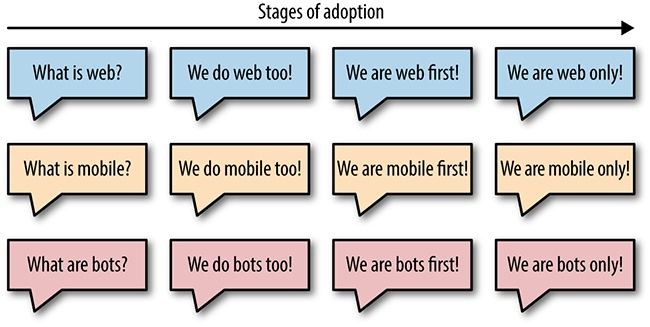
\includegraphics[scale=.3]{images/four-phases-of-adoption}
			\label{trello}
		\end{figure}
		\item Bots are going to disrupt the software industry in the same way the web and mobile revolutions did.
		% bots have been the subject of immense excitement in the belief that they might replace mobile apps for many tasks and provide a flexible and natural interface for sophisticated AI technology.
	\end{itemize}
\end{frame}

\begin{frame}
	\frametitle{Motivation}
	\framesubtitle{Accelerators}
	\begin{itemize}
		\item The mobile app economy is stagnating.
		% it’s getting harder to persuade consumers to download and use new apps, 
		% and even once they’re installed it’s hard to get users to return to them. 
		% As recently noted in The Economist: The 20 most successful developers grab nearly half of all revenues on Apple’s App Store. 
		% Building apps and promoting them is getting more costly. 
		% Meanwhile, users’ enthusiasm is waning, as they find downloading apps and navigating between them a hassle. 
		% A quarter of all downloaded apps are abandoned after a single use.
		% Pew Research Center, most apps aren’t kept longer than a day after users download them. 
		% Just over 3\% of apps are still active 30 days after being downloaded.
		\item Consumers like conversational interfaces.
		%, and companies want to make themselves available on the platforms that their customers enjoy using. 
		% Facebook Messenger is the most popular Android app; 
		% it and WhatsApp (another Facebook messaging app) each have more than one billion active users on Android alone. 
		% Consumers spend more than 4 hours per week in communication apps, according to Nielsen. 
		% More than half of WhatsApp users use the app more than once a day; over 80\% use it at least once daily. 
		% Line is similarly dominant in Japan, 
		% as is WeChat in China.
		\item Bots are the ultimate source of cheap labor.
		% If you’re running a customer contact center, you’re probably already considering the idea of using bots to replace or augment human workers. 
		% the cost of servicing customers with humans is high. 
		% Lower-cost customer service could mean more customer service. 
		% And since the bots will have access to much more information than any human worker could possibly have, ideally, the bot will “know” the answer to your question before you even ask it.
		\item Make workers more productive by taking care of time-consuming repetitive tasks.
		% But bots aren’t just about replacing workers. 
		% They promise to make workers more productive by taking care of time-consuming repetitive tasks like scheduling meetings, coordinating team discussions, and updating databases.
		% Nearly any simple, well-defined human office task could be addressed by a bot, freeing humans for more complex work.
		\item AI has advanced remarkably in the last few years.
		% and is reaching the point where computers can have moderately complex conversations with users in natural language. 
		% Plus, AI-as-a-service is beginning to become available, making it possible for developers without deep learning expertise to implement AI in their software.
		% Deep learning is one of the enabling developments in artificial intelligence that has enabled the rise of bots. 
	\end{itemize}
\end{frame}

\begin{frame}
	\frametitle{Motivation}
	\framesubtitle{Competition}
	\begin{figure}[h]
		\centering
		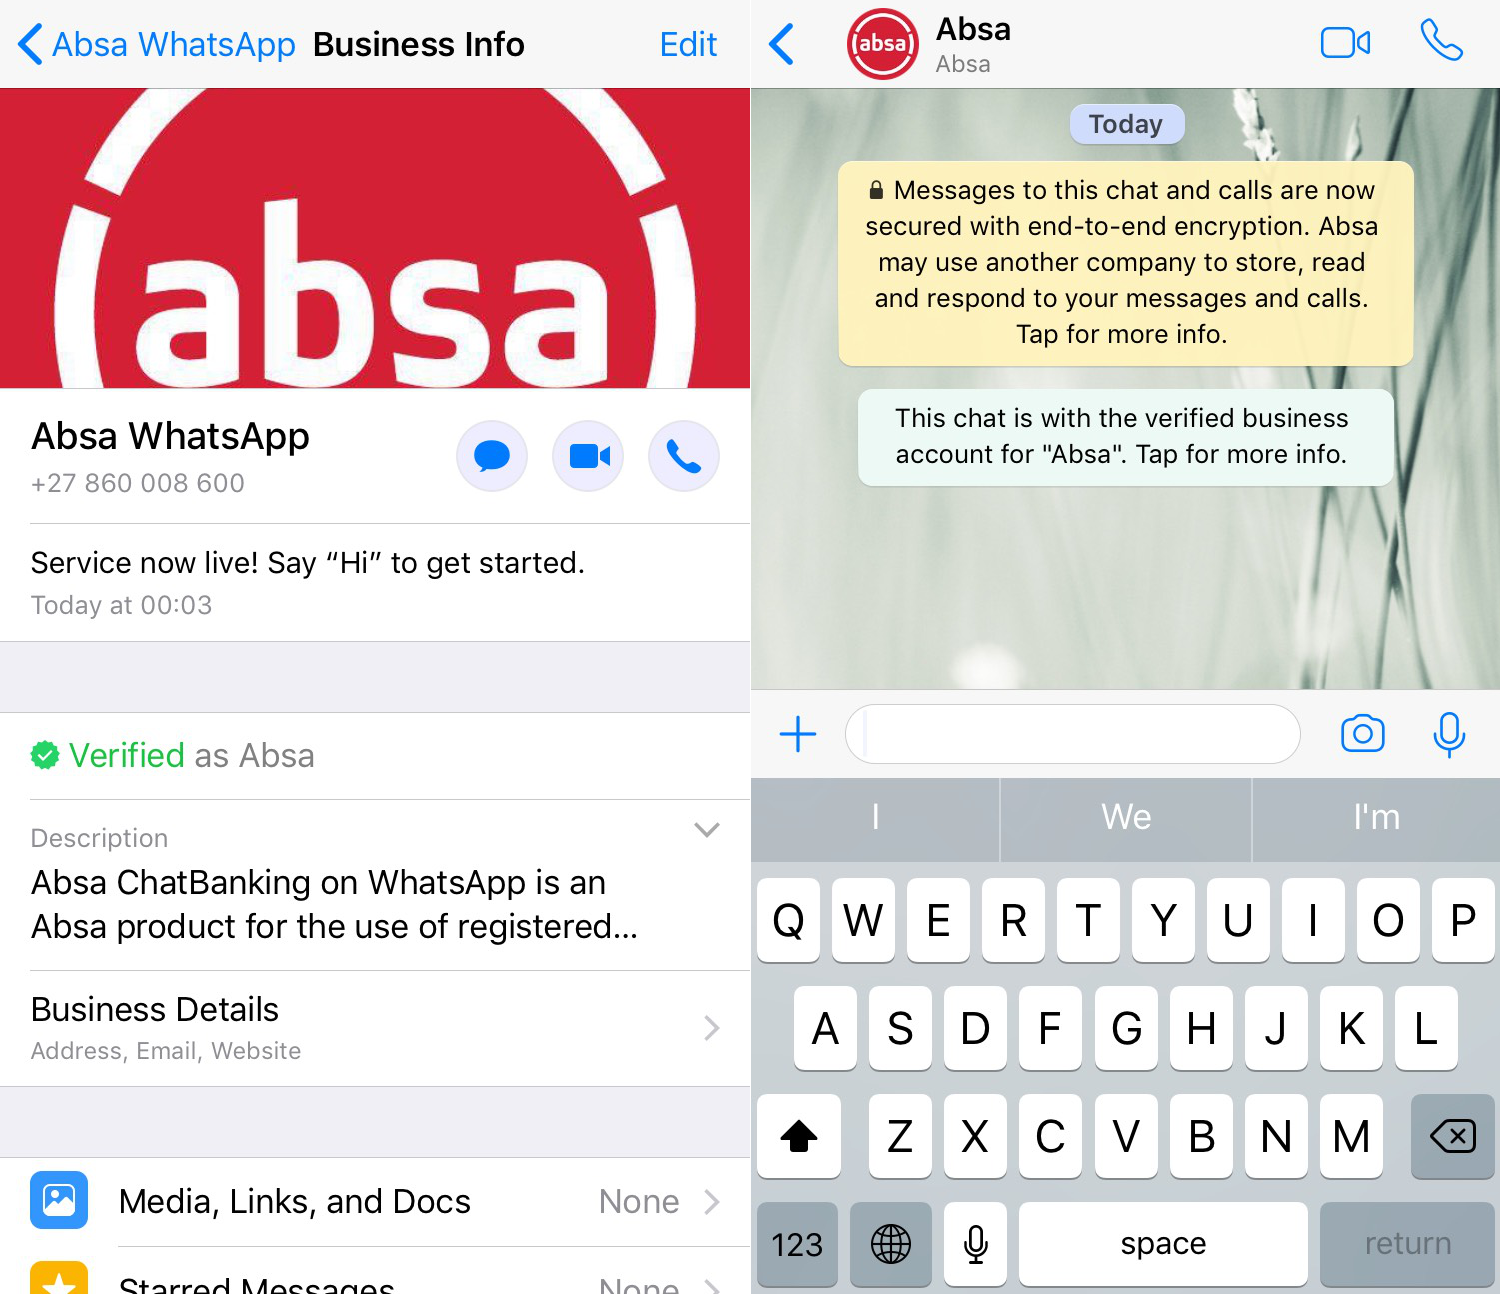
\includegraphics[scale=.15]{images/Absa-Whatsapp}
		\label{Absa-Whatsapp}
	\end{figure}
\end{frame}

\begin{frame}
	\frametitle{Motivation}
	\framesubtitle{Competition}
	\begin{figure}
		\centering
		\subfloat[Start]{{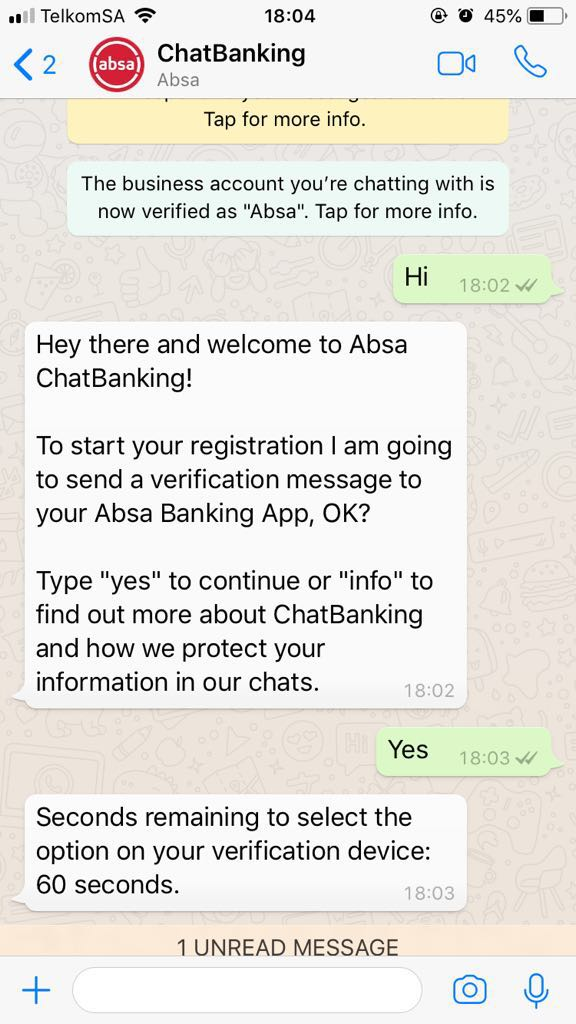
\includegraphics[width=5cm, height=7cm]{images/sithole1} }}%
		\qquad
		\subfloat[Continue]{{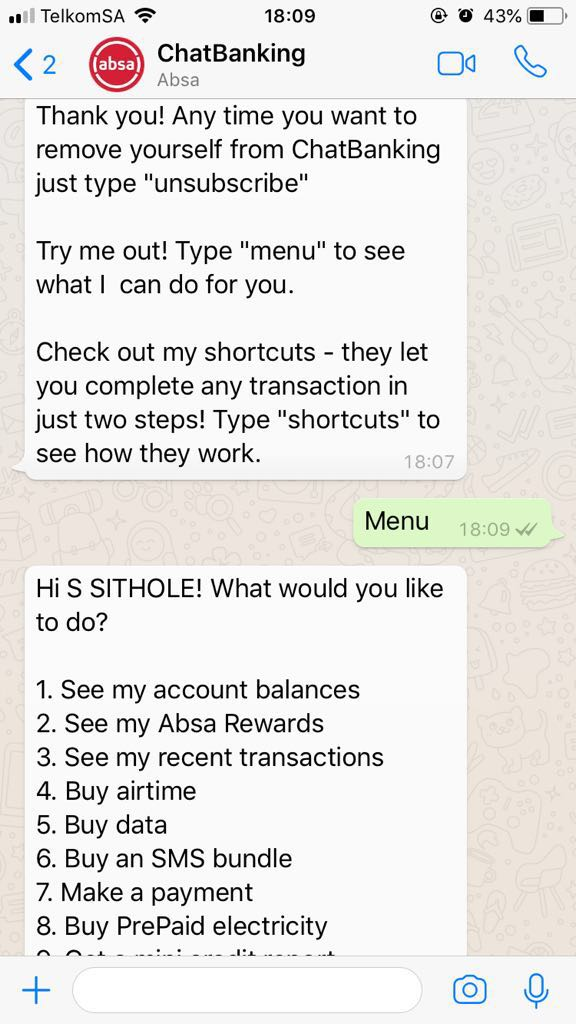
\includegraphics[width=5cm, height=7cm]{images/sithole2} }}%
	\end{figure}

\end{frame}

\begin{frame}
	\frametitle{Motivation}
	\framesubtitle{Competition}
	\begin{itemize}
		\item WhatsApp Pay services:
		\begin{itemize}
			\item Absa is the first to fully launch WhatsApp Pay services anywhere in the world.
			\item A number of banking institutions in India have trialled using the platform for banking services.
			% notably private lender Kotak Mahindra Bank,  
		\end{itemize}
		\item Absa ChatBanking:
		\begin{itemize}
			\item Facebook Messenger, Twitter, WhatsApp.
			\item Check bank balance, buy electricity, purchase airtime and data, pay beneficiaries.
		\end{itemize}
		% To use WhatApp banking, you need to follow these steps:
		% Add Absa (086 000 8600) as a contact on your device;
		% Open WhatsApp and find the new contact;
		% Simply say ‘hi’ to your Absa contact.
	\end{itemize}
\end{frame}


\begin{frame}
	\frametitle{Definition}
	\framesubtitle{What exactly is a bot?}
	\begin{itemize}
		\item Bots are AI-driven pieces of software that converse in human terms.
		\item NLP is the discipline concerned with making computers communicate in human terms.
	%	\item They’re not quite ready to pass the Turing test, but ready enough for many forms of commerce and messaging.
	%	\item Bots are able to automate human tasks for which APIs don’t exist, translating fluidly between unstructured language and structured data.
		\item AI makes it possible for bots to parse human language, understand intent, and compose replies. 
		% AI of some sort is a key component of most bots, 
		% but many bots also have humans underneath them — this is called “human in the loop.” 
		% Bots may rely on humans to train them, 
		% or bots may act as filters and qualifiers, gathering information to help humans work more effectively.
		\item Bots communicate in human language through a variety of interfaces.
		% — IM, email, and voice are the platforms of greatest interest now. 
		% This is a crucial aspect because bots can reach their users anywhere, and they’re easy to install; 
		% instead of downloading a new app, you just add a new contact in your IM client.
		% And unlike apps, which are almost all subject to the control of Apple and Google, the field for bots is much more open (for now, at least).
	\end{itemize}
\end{frame}

\begin{frame}
\frametitle{Definition}
\framesubtitle{How are bots different from humans?}
\begin{itemize}
		\item Bots have no online status and no last seen timestamps.
		%, the interface shows the label ‘bot’ instead.
		\item Bots have limited cloud storage.
		% — older messages may be removed by the server shortly after they have been processed.
		\item Bots can't initiate conversations with users.
		% A user must either add them to a group or send them a message first. 
		% People can use telegram.me/<bot\_username> links or username search to find your bot.
		\item Bot usernames always end in ‘bot’.
		% (e.g. @TriviaBot, @GitHub\_bot).
		\item When added to a group, bots do not receive all messages by default.
\end{itemize}
\end{frame}

\begin{frame}
	\frametitle{Types}
	\begin{itemize}
		\item Personal vs. team bots
		\item Super bots vs. domain-specific bots
		\item Business bots vs. consumer bots
		\item Voice vs. text bots % (Slack and Facebook Messenger vs Amazon Echo and Google Assistant)
		\item Net new bots vs. integrations exposing legacy systems
	\end{itemize}
\end{frame}

%\begin{frame}
%	\frametitle{Definitions}
%	\begin{itemize}
%		\item Several of these stacks also offer a central AI agent like Siri, Google Now, or Alexa that ties services together and could eventually operate as a “god bot” that dispatches work to other bots (for instance, opening the Uber bot when you say “Alexa, call me a car.”)
%		\item The discipline of bot UI design is brand new, and significantly different from traditional web UI design.
%	\end{itemize}
%\end{frame}


\begin{frame}
	\frametitle{Applications}
	\begin{itemize}
		\item Conversational Commerce
		\item Bots for Business
		\item Productivity and Coaching
		\item Alert and Notification Bots
		\item Bots as Routers between Humans
		\item Customer Service and FAQ Bots
		\item Third Party Integration Bots
		\item Games and Entertainment Bots
		\item Brand Bots
		% Customer relationship management - Consumer-facing bots can assist customers with difficult transac‐ tions, make recommendations, and gather data. For instance, a bot incorporated into an airline’s website could answer questions about fees, rebook flights, and suggest add-ons like hotel and car reserva‐ tions. Even if the bot isn’t able to finish these exchanges, it could still gather preliminary information (customer’s name, reservation num‐ ber, etc.) and pass it on to a customer service representative, saving considerable time for the company’s call center. Matched to a sophisticated data-mining backend, the bot builds up data profiles that the airline can use to market vacations, travel deals, and addi‐ tional services.
		% - Specialized bots can make professional tasks easier. For instance, a bot connected to an electronic medical record system could retrieve information faster than a conventional lookup; just ask “what was the patient’s blood pressure during his January visit?”
		% Productivity bots like x.ai are already able to schedule meetings through email, posing as a human assistant.
		% - Bots can take advantage of the intimate, low-friction environment of messaging to provide coaching, healthy reminders, or entertainment. For instance, a wellness bot, popping up inside the IM client that you’re accustomed to using all day, could encourage you to exercise or meditate. Game bots are already widespread.
		% Customer care - Improve customer relations and reduce cost by up to 40 percent. Investing in AI technology can effectively upskill your agents, streamline how you engage with customers, partners and employees. Watson offers a virtual assistant solution to transform your customer service department.
		% Automotive - digital assistant designed to enhance in-vehicle experiences, helping the automotive industry better understand and interact with drivers and passengers.
		% Hospitality - offers a customized digital assistant to provide a differentiated and personalized experience for hotel guests.
		% Tradeoff Analytics
		% Investment Advisor
	\end{itemize}
\end{frame}

\begin{frame}
\begin{center}
	PART II \\ Technology Providers
\end{center}
\end{frame}

\begin{frame}
\frametitle{Overview of Bots Landscape}
\begin{figure}[h]
	\centering
	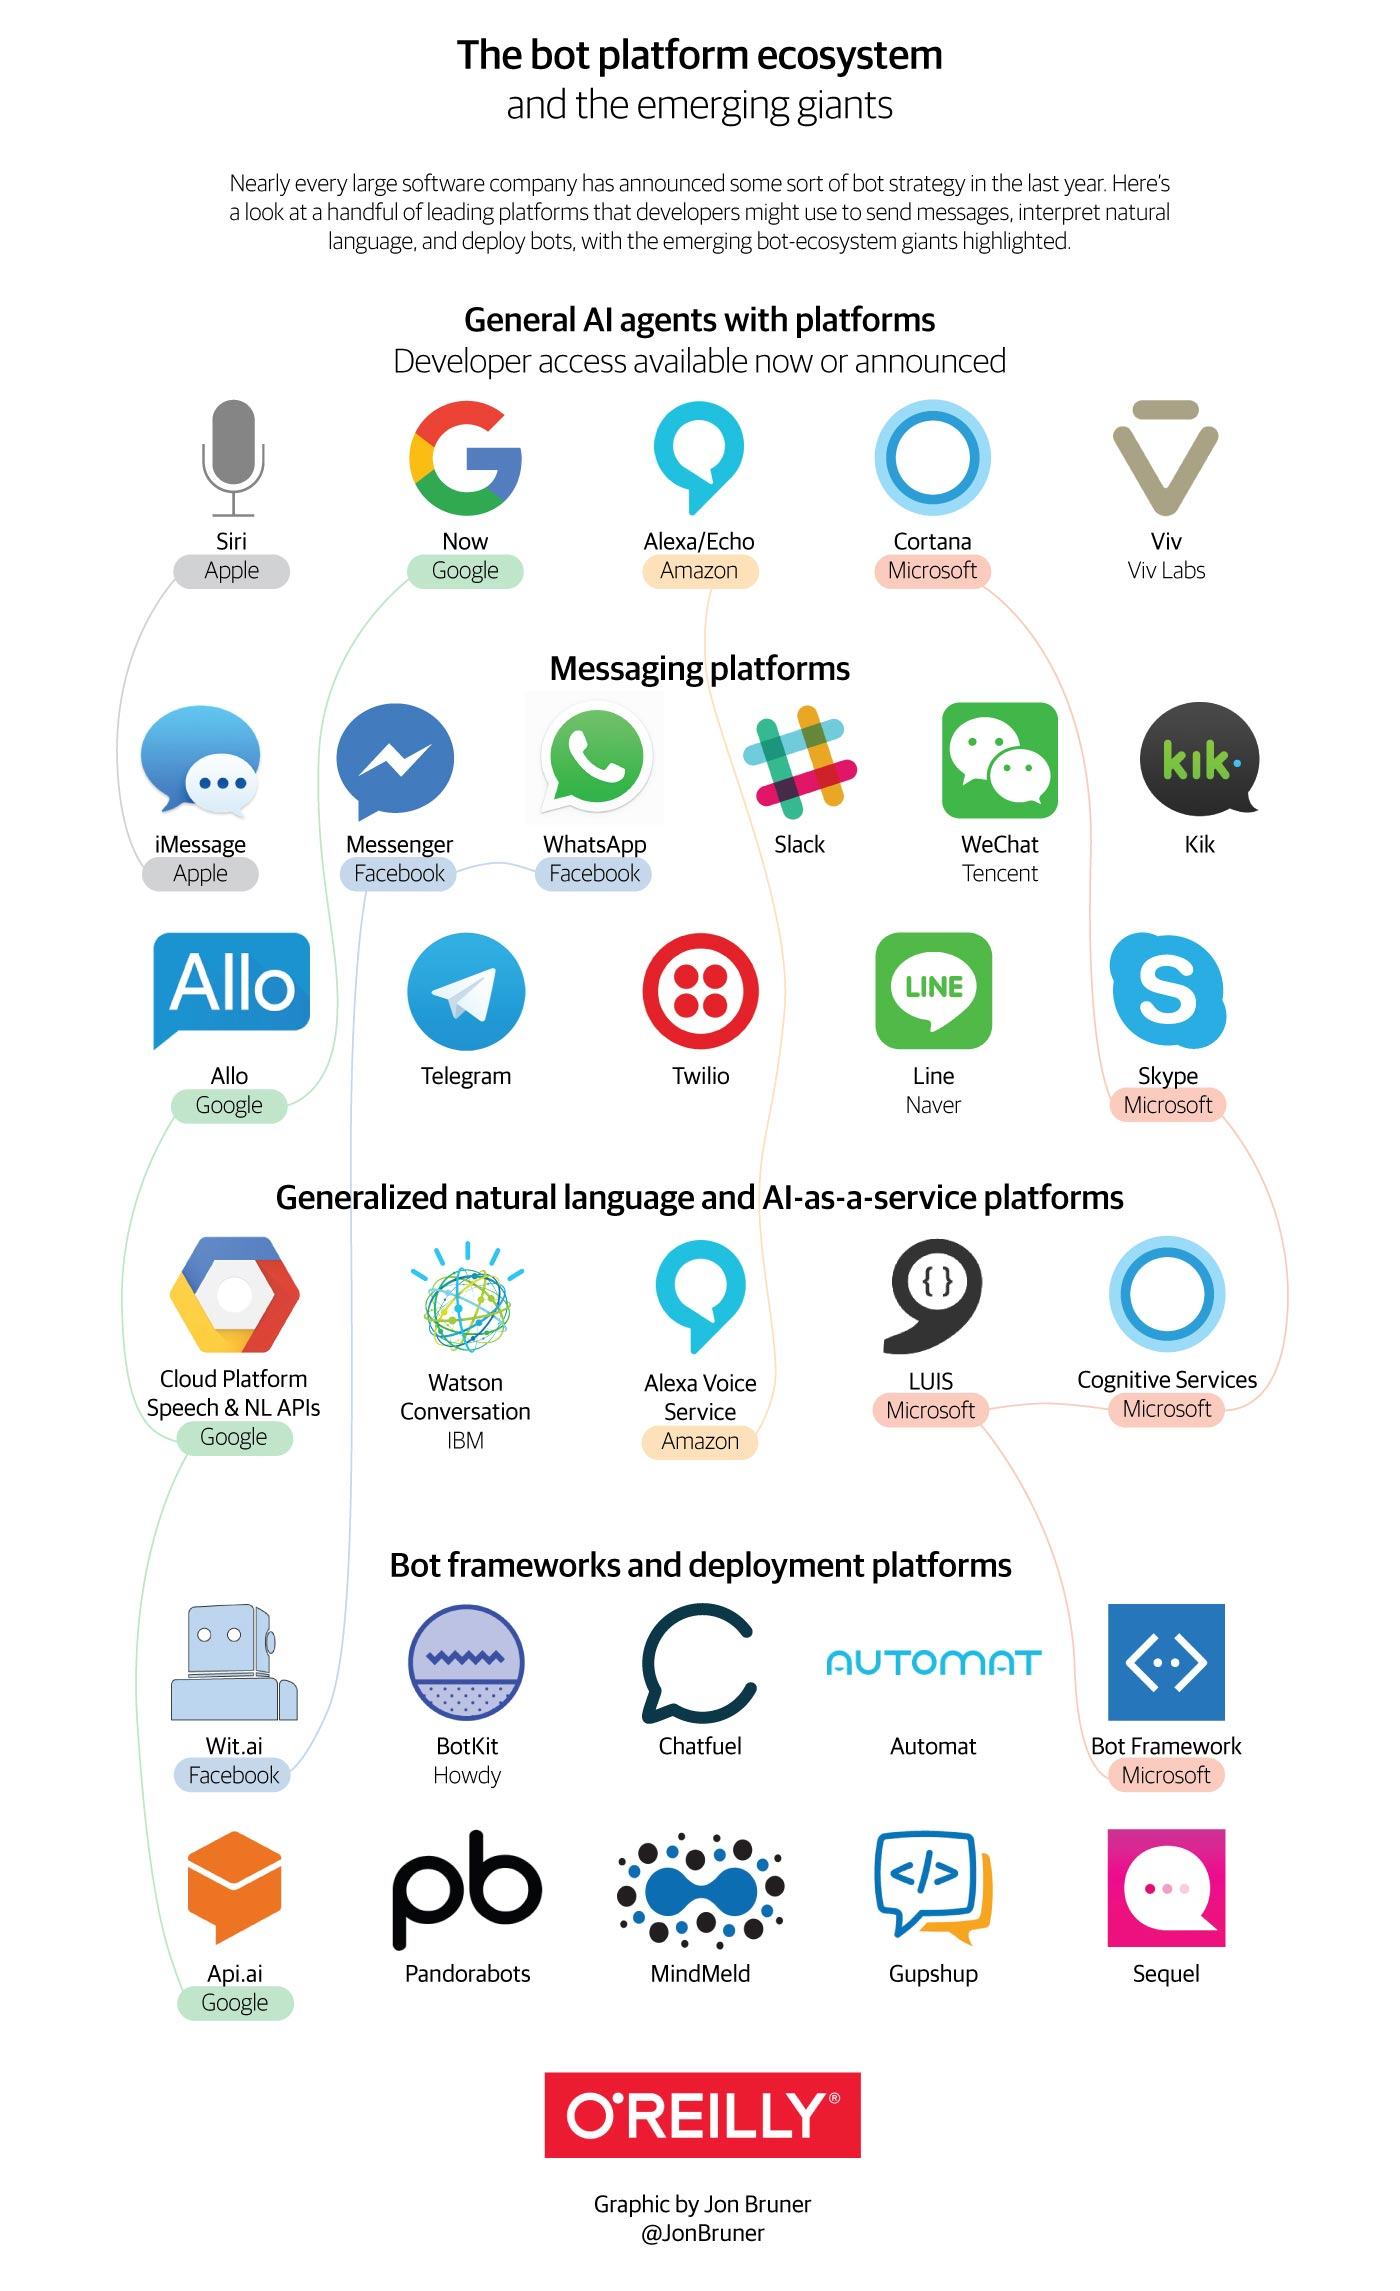
\includegraphics[scale=.1]{images/bots-landscape-2017}
\end{figure}
\end{frame}

\begin{frame}
\frametitle{General AI Agents with Platforms}
\begin{figure}[h]
	\centering
	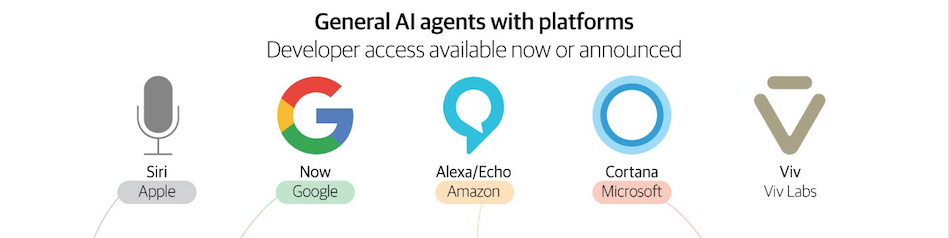
\includegraphics[scale=.5]{images/gen-ai-agents}
\end{figure}

\end{frame}

\begin{frame}
\frametitle{Messaging Platforms}
\begin{figure}[h]
	\centering
	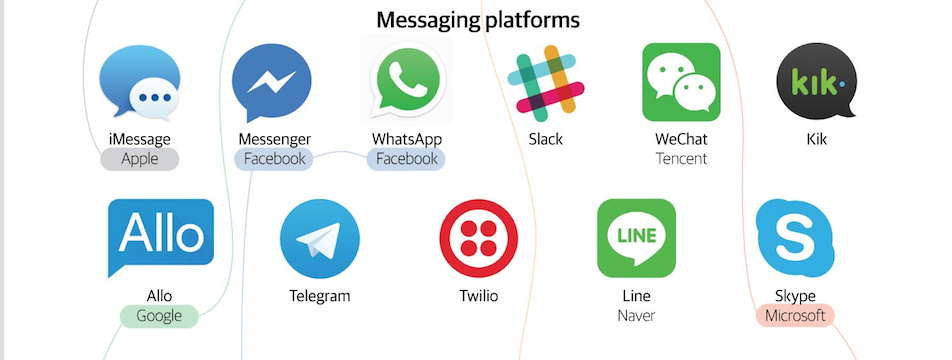
\includegraphics[scale=.5]{images/messaging-platforms}
\end{figure}
Where bots live.
\end{frame}

\begin{frame}
\frametitle{Generalized NL and AI-as-a-Service Platforms}
\begin{figure}[h]
	\centering
	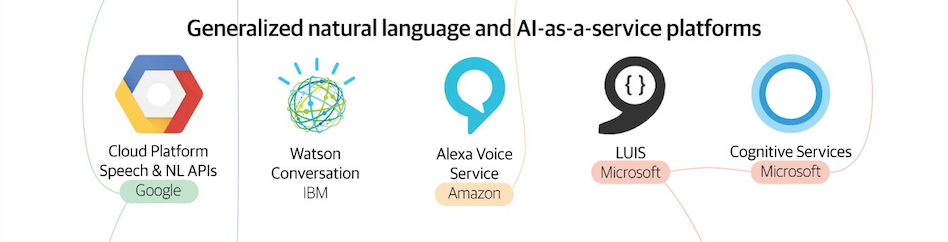
\includegraphics[scale=.5]{images/ai-as-a-service}
\end{figure}
The sophistication of a bot is directly linked to the sophistication of its AI model. AI as a service makes it easy to implement very basic AI.
\end{frame}

\begin{frame}
\frametitle{Bot Frameworks and Deployment Platforms}
\begin{figure}[h]
	\centering
	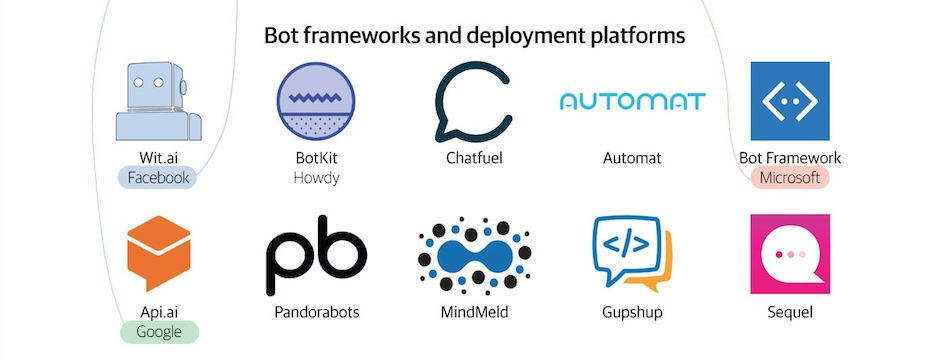
\includegraphics[scale=.5]{images/bot-frameworks}
\end{figure}
Tools, platforms, and resources that make it easy to deploy chatbots.
\end{frame}


\begin{frame}
\frametitle{References}
\begin{enumerate}
	\item What are Conversational Bots? An Introduction to and Overview of AI-Driven Chatbots by Jon Bruner and Mike Barlow (2016)
	\item Designing Bots by Amir Shevat (2017)
\end{enumerate}
\end{frame}

%\begin{frame}
%\frametitle{Telegram}
%\begin{enumerate}
%	\item Bots are third-party applications that run inside Telegram. Users can interact with bots by sending them messages, commands and inline requests. You control your bots using HTTPS requests to our bot API.
%	\item At the core, Telegram Bots are special accounts that do not require an additional phone number to set up. Users can interact with bots in two ways:
%		\begin{itemize}
%		\item Send messages and commands to bots by opening a chat with them or by adding them to groups.
%		\item Send requests directly from the input field by typing the bot's @username and a query. This allows sending content from inline bots directly into any chat, group or channel.
%	\end{itemize}
%\end{enumerate}
%\end{frame}
%
%\begin{frame}
%\frametitle{Telegram}
%\begin{enumerate}
%	\item You could use bots to:
%	\begin{itemize}
%		\item Get customized notifications and news. A bot can act as a smart newspaper, sending you relevant content as soon as it's published.
%		TechCrunch Bot
%		\item Integrate with other services. A bot can enrich Telegram chats with content from external services.
%		Gmail Bot, Image Bot, GIF bot, IMDB bot, Wiki bot, Music bot, Youtube bot, GitHub bot
%		\item Accept payments from Telegram users. A bot can offer paid services or work as a virtual storefront. Read more »
%		Demo Shop Bot
%		\item Create custom tools. A bot may provide you with alerts, weather forecasts, translations, formatting or other services.
%		Markdown bot, Sticker bot, Vote bot, Like bot
%		\item Build single- and multiplayer games. A bot can offer rich HTML5 experiences, from simple arcades and puzzles to 3D-shooters and real-time strategy games.
%		GameBot, Gamee
%		\item Build social services. A bot could connect people looking for conversation partners based on common interests or proximity.
%		HotOrBot
%	\end{itemize}
%\end{enumerate}
%\end{frame}
%
%\begin{frame}
%\frametitle{Telegram}
%\begin{enumerate}
%	\item At the core, Telegram Bots are special accounts that do not require an additional phone number to set up. Users can interact with bots in two ways:
%	\begin{itemize}
%		\item Send messages and commands to bots by opening a chat with them or by adding them to groups.
%		\item Send requests directly from the input field by typing the bot's @username and a query. This allows sending content from inline bots directly into any chat, group or channel.
%	\end{itemize}
%	\item To create a bot, talk to BotFather and follow a few simple steps.
%	\item Once you've created a bot and received your authorization token, head down to the Bot API manual to see what you can teach your bot to do.
%	\item Telegram bots are unique in many ways — we offer two kinds of keyboards, additional interfaces for default commands and deep linking as well as text formatting
%\end{enumerate}
%\end{frame}
%
%\begin{frame}
%\frametitle{Telegram}
%\begin{enumerate}
%	\item Telegram bots are unique in many ways — we offer two kinds of keyboards, additional interfaces for default commands and deep linking as well as text formatting.
%	\begin{itemize}
%		\item Inline mode
%		\item Payments platform
%		\item Gaming platform
%		\item Keyboards
%		\item Inline keyboards and on-the-fly updating
%		\item Commands
%		\item Global commands
%		\item Privacy mode
%		\item Deep linking
%		\item Location and Number
%	\end{itemize}
%\end{enumerate}
%\end{frame}
%
%\begin{frame}
%\frametitle{Telegram}
%\begin{itemize}
%	\item BotFather is the one bot to rule them all. It will help you create new bots and change settings for existing ones.
%	\begin{itemize}
%		\item Creating a new bot
%		\item Generating an authorization token
%		\item List your bots
%		\item List your games
%		\item Edit bot name, description, set bot profile picture, supported commands, delete a bot.
%		\item Status alerts
%		\item Responding to alerts
%		\item Monitoring issues
%	\end{itemize}
%\end{itemize}
%\end{frame}


%\begin{frame}
%\frametitle{Slack}
%\begin{enumerate}
%	\item Enable conversations between users and apps in Slack by building bots.
%	\item A bot is a type of Slack App designed to interact with users via conversation.
%	\item A bot is the same as a regular app: it can access the same range of APIs and do all of the magical things that a Slack App can do.
%	\item But when you build a bot for your Slack App, you're giving that app a face, a name, and a personality, and encouraging users to talk to it.
%	\item Your bot can send DMs, it can be mentioned by users, it can post messages or upload files, and it can be invited to channels - or kicked out.
%\end{enumerate}
%\end{frame}
%
%

\end{document}